\section{Leggi di controllo}
In questa sezione verranno accennati diversi modelli di controlli utilizzati odiernamente per controllare i quadricotteri, \cite{ZuluAndrew2014ARoC}, \cite{KimJinho2020ACSo}. Questi si possono classificare in tre categorie come in figure \ref{fig:categoriecontrolli}.
\begin{figure}
	\centering
	\includegraphics[width=0.6\textwidth]{SistemaQuadrirotore/Figure/Classificazione}
	\caption{Classificazione dei titpi di controllori maggiormente utilizzati}
	\label{fig:categoriecontrolli}
\end{figure}

\subsection{Controllori Lineari}
\subsubsection{Controllore Proportional-Integral-Derivative Controller (PID)}
Il controllore PID è molto utilizzato in diverse applicazioni, la sua semplicità e facilità di impostazione dei parametri lo rende molto rapido da implementare e relativamente robusto. Inoltre non è necessario avere la misura dello stato completo del sistema da controllare, per funzionare, semplificando eventualmente la determinazione di questo. Il principale problema risiede nella risposta alle eventuali non linearità presenti nel modello del sistema controllato o nella realtà.

\begin{figure}
	\centering
	\includegraphics[width=0.6\textwidth]{SistemaQuadrirotore/Figure/PID}
	\caption{Schema di applicazione del controllore PID}
\end{figure}

\subsubsection{Controllore Linear Quadratic Regulator (LQR)}
Questo tipo di controllore si ottiene la minimizzazione della funzione di costo, ottenendo una matrice di guadagni con la quale si applica il controllo in retroazione. A differenza del PID, questo tipo di controllo prevede di avere tutto il vettore di stato a disposizione. per questo motivo viene accompagnato spesso da un Linear Quadratic Estimator (LQE) ed un filtro di Kalman, con lo scopo di determinare dalle misurazioni dei sensori lo stato del sistema. Il metodo utilizzato per determinare la matrice dei guadagni è un aspetto molto importante, inoltre è necessario modellare in modo molto preciso il sistema controllato per evitare di trovare una soluzione poco soddisfacente. Questo tipo di controllo può essere specializzato per ottenere una soluzione ottima di risparmio della batteria \cite{KoksalN2018ALQA}, risultando però poco robusti \cite{ZuluAndrew2014ARoC}.

\begin{figure}
	\centering
	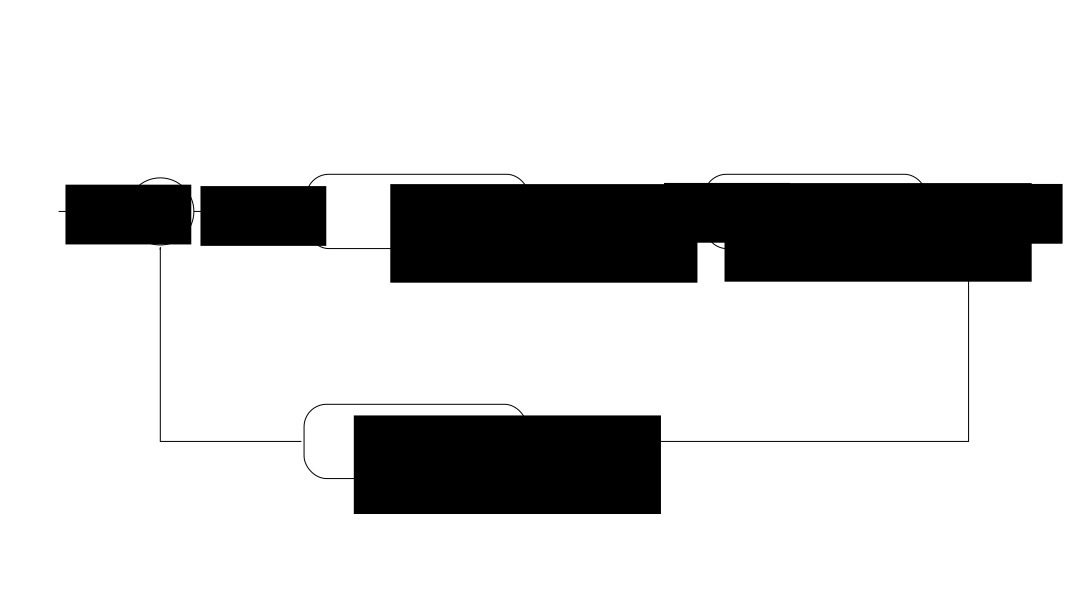
\includegraphics[width=0.6\textwidth]{SistemaQuadrirotore/Figure/LQR}
	\caption{Schema di applicazione del controllore LQR}
\end{figure}
 

\subsubsection{Controllore $H_\infty$}

Il controllore $H_\infty$ si ottiene esprimendo la soluzione del controllo attraverso una formulazione matematica, prende il nome dallo spazio matematico in cui ha luogo l'ottimizzazione, ovvero lo spazio di Hardy. Il problema principale di questo approccio è la complessità analitica che risiede nell'ottimizzazione stessa. Il sistema così trovato però ha il vantaggio di essere di più facile implementazione su sistemi multi-variabili. 

\subsection{Controllori non lineari}

\subsubsection{Controllore con Feedback Linearization}

Questo tipo di controllore viene utilizzato comunemente. La logica di funzionamento prevede di utilizzare un controllo lineare prestante. Introducendo una mappatura dell'ingresso al sistema, attuando di fatto un cambiamento di variabili di controllo, si fa in modo che il sistema lienare sia in grado di controllare il sistema controllato efficacemente. Il controllo lineare comanda quindi un sistema linearizzato equivalente al sistema non lineare. Questo tipo di approccio ha lo svantaggio però di essere molto sensibile alle incertezze e i rumori dei sensori, fattore che ne inficia la robustezza.

\begin{figure}
	\centering
	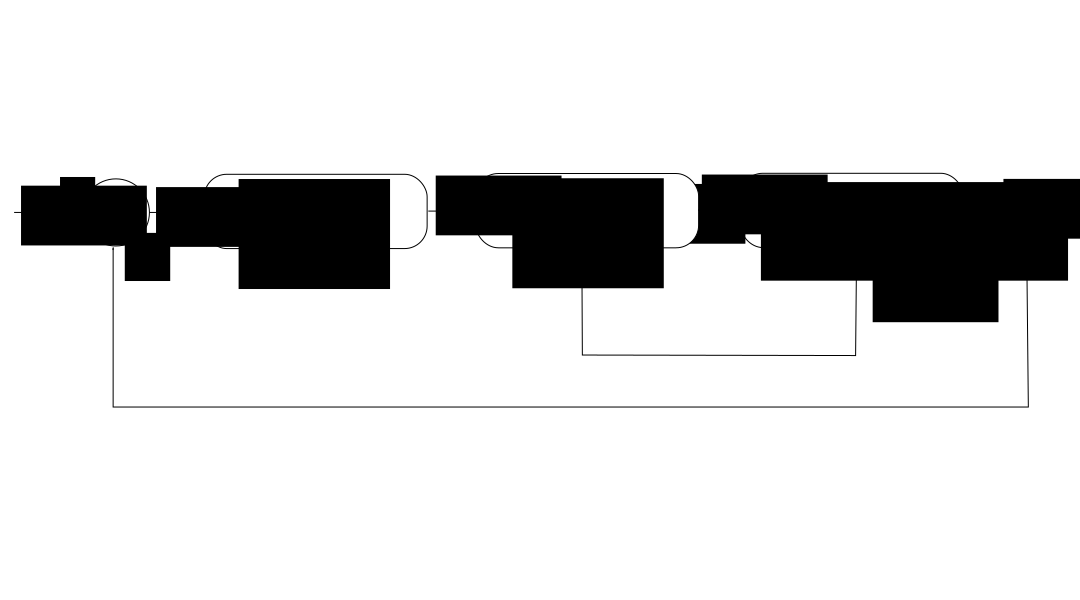
\includegraphics[width=0.6\textwidth]{SistemaQuadrirotore/Figure/FLP}
	\caption{Schema di applicazione del controllore con Feedback Linearization}
\end{figure}

\subsubsection{Controllore con Backstepping}

Si basa su di un algoritmo ricorsivo che segmenta il controllore in sottoparti, stabilizzando queste parti in modo progressivo. Questo tipo di controllore ha una procedura di convergenza molto rapida. Il suo difetto maggiore è la poca robustezza. Per poter migliorare la risposta può essere aggiunto un integratore con l'obbiettivo di ridurre l'errore stazionario.


\subsubsection{Controllore Sliding Mode Control (SMC)}

Questo tipo di controllo prevede di utilizzare un segnale di comando discontinuo, la legge di controllo non è quindi continua nel tempo. Questo sistema risulta essere molto preciso e robusto, come verrà mostrato nelle simulazioni successive. A causa della discontinuità introdotta si può  osservare il fenomeno di chattering, che ha come effetto secondario l'aumento dell'utilizzo degli attuatori, ovvero un maggior consumo di batteria. Questo effetto può essere mediato applicando alcuni filtri in uscita dal controllore, che mediano le discontinuità. Il controllo basa il funzionamento sulla definizione di una superfice di sliding definita dallo stato del sistema, una volta portato su questa superficie attraverso il segnale discontinuo il controllore mantiene le oscillazioni nei dintorni di questa. Questo tipo di controllore è molto robusto e si comporta bene in presenza di rumore ed incertezze come l'effetto suolo.

\begin{figure}
	\centering
	\includegraphics[width=0.6\textwidth]{SistemaQuadrirotore/Figure/SMC}
	\caption{Schema di applicazione del controllore SMC}
\end{figure}

\subsection{Controllori intelligenti}

\subsubsection{Controllore con Modello predittivo (MPC)}

Questo tipo di controllo si basa sulla previsione dello stato e del comando che verrà attuato seguendo dei modelli previsionali e stimatori. Molto utile se si vuole evitare di superare alcune imposizioni specifiche (forzare input e output in determinati contorni).
E' necessario un buon stimatore. Il controllore è in grado di reagire efficacemente in presenza di guasti ai motori.

\begin{figure}
	\centering
	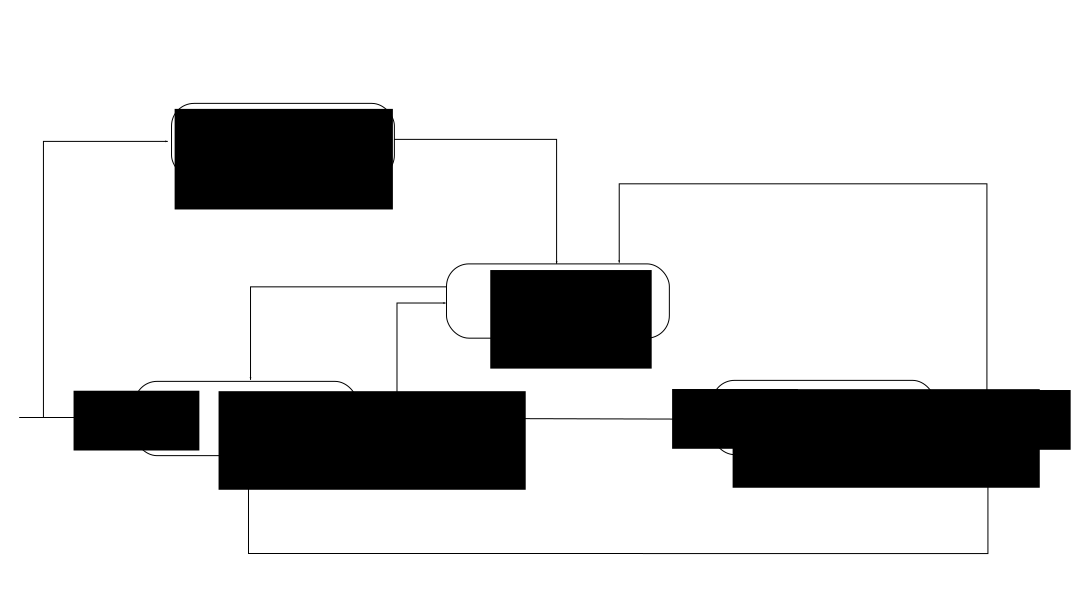
\includegraphics[width=0.6\textwidth]{SistemaQuadrirotore/Figure/MPC}
	\caption{Schema di applicazione del controllore MPC}
\end{figure}

\subsubsection{Controllore con logica Fuzzy}

Questo tipo di controllo si basa sulla presenza di stati logici non binari, range di valori  . Una serie di verifiche di condizioni soddisfatte con eventuali azionamenti specifici seguendo un algoritmo. Ad ogni passaggio il segnale di uscita viene determinando tenendo conto di diversi step per poter essere mandato al velivolo controllato. Non richiedono una conoscenza completa del sistema.

\begin{figure}
	\centering
	\includegraphics[width=0.8\textwidth]{SistemaQuadrirotore/Figure/Fuzzy}
	\caption{Schema di applicazione del controllore Fuzzy}
\end{figure}

\subsubsection{Controllore con Neural Network}

Si utilizza una rete neurale formata da diversi layer con la quale attraverso una fase di addestramento si ottiene un sistema di controllo. La rete è formata da neuroni collegati attraverso dei collegamenti pesati. Il vantaggio di questo metodo di controllo è la capacità di avere risultati migliori rispetto ai normali controlli lineari senza dover necessariamente conoscere la dinamica del quadrirotore e i suoi parametri.

\begin{figure}
	\centering
	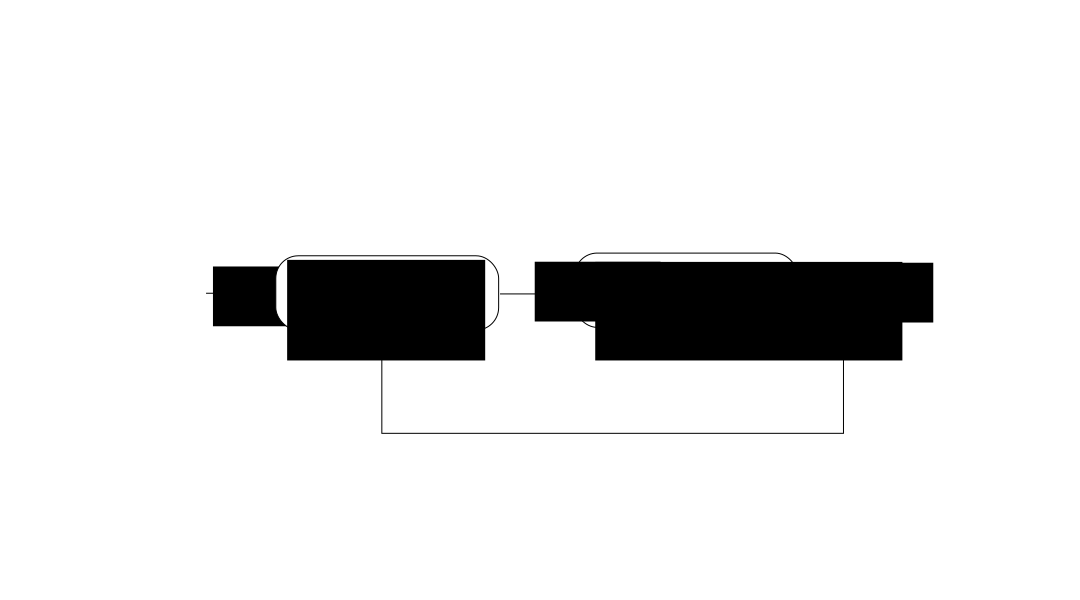
\includegraphics[width=0.6\textwidth]{SistemaQuadrirotore/Figure/NN}
	\caption{Schema di applicazione del controllore con Neural Network}
\end{figure}
